%\documentclass[tikz,border=2mm]{standalone}
\documentclass[tikz,border=2mm]{standalone}
\usepackage{amssymb}
\usepackage{amsmath}

\begin{document}

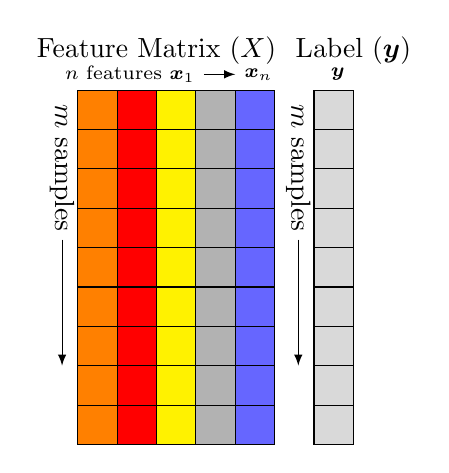
\begin{tikzpicture}[>=latex,every node/.style={minimum size=.5cm-\pgflinewidth, outer sep=0pt}]
   \draw [fill=orange] (0.0,0.0) rectangle (0.5,4.5);
   \draw [fill=red] (0.5,0.0) rectangle (1.0,4.5);
   \draw [fill=yellow] (1.0,0.0) rectangle (1.5,4.5);  
   \draw [fill=gray!60] (1.5,0.0) rectangle (2.0,4.5);  
    \draw [fill=blue!60] (2.0,0.0) rectangle (2.5,4.5);  
    \draw[step=0.5cm,color=black] (0,0) grid (2.5,4.5);
    \node at (1,5.0) {Feature Matrix ($X$)};
    %\node at (1,4.7) {\scriptsize{$n$ features $\boldsymbol{x}_1\longrightarrow \boldsymbol{x}_n$}};
    \draw[->] (1.6,4.7) node [left] {\scriptsize{$n$ features $\boldsymbol{x}_1$}} -- (2,4.7)  node[right] {\scriptsize{$\boldsymbol{x}_n$}};
    \node[label=below:\rotatebox{-90}{ $m$ samples }] at (-0.2,4.8) {};
    \draw[->] (-0.2, 2.6) -- (-0.2,1);
    
    \draw [fill=gray!30] (3.0,0.0) rectangle (3.5,4.5);
     \draw[step=0.5cm,color=black] (3.0,0) grid (3.5,4.5);  
     \node[label=below:\rotatebox{-90}{ $m$ samples }] at (2.8,4.8) {};
     \node at (3.5,5.0) {Label ($\boldsymbol{y}$)};
      \node at (3.3,4.7) {\scriptsize{$\boldsymbol{y}$}};
      \draw[->] (2.8, 2.6) -- (2.8,1);
\end{tikzpicture}

\end{document}